\documentclass[1p]{elsarticle_modified}
%\bibliographystyle{elsarticle-num}

%\usepackage[colorlinks]{hyperref}
%\usepackage{abbrmath_seonhwa} %\Abb, \Ascr, \Acal ,\Abf, \Afrak
\usepackage{amsfonts}
\usepackage{amssymb}
\usepackage{amsmath}
\usepackage{amsthm}
\usepackage{scalefnt}
\usepackage{amsbsy}
\usepackage{kotex}
\usepackage{caption}
\usepackage{subfig}
\usepackage{color}
\usepackage{graphicx}
\usepackage{xcolor} %% white, black, red, green, blue, cyan, magenta, yellow
\usepackage{float}
\usepackage{setspace}
\usepackage{hyperref}

\usepackage{tikz}
\usetikzlibrary{arrows}

\usepackage{multirow}
\usepackage{array} % fixed length table
\usepackage{hhline}

%%%%%%%%%%%%%%%%%%%%%
\makeatletter
\renewcommand*\env@matrix[1][\arraystretch]{%
	\edef\arraystretch{#1}%
	\hskip -\arraycolsep
	\let\@ifnextchar\new@ifnextchar
	\array{*\c@MaxMatrixCols c}}
\makeatother %https://tex.stackexchange.com/questions/14071/how-can-i-increase-the-line-spacing-in-a-matrix
%%%%%%%%%%%%%%%

\usepackage[normalem]{ulem}

\newcommand{\msout}[1]{\ifmmode\text{\sout{\ensuremath{#1}}}\else\sout{#1}\fi}
%SOURCE: \msout is \stkout macro in https://tex.stackexchange.com/questions/20609/strikeout-in-math-mode

\newcommand{\cancel}[1]{
	\ifmmode
	{\color{red}\msout{#1}}
	\else
	{\color{red}\sout{#1}}
	\fi
}

\newcommand{\add}[1]{
	{\color{blue}\uwave{#1}}
}

\newcommand{\replace}[2]{
	\ifmmode
	{\color{red}\msout{#1}}{\color{blue}\uwave{#2}}
	\else
	{\color{red}\sout{#1}}{\color{blue}\uwave{#2}}
	\fi
}

\newcommand{\Sol}{\mathcal{S}} %segment
\newcommand{\D}{D} %diagram
\newcommand{\A}{\mathcal{A}} %arc


%%%%%%%%%%%%%%%%%%%%%%%%%%%%%5 test

\def\sl{\operatorname{\textup{SL}}(2,\Cbb)}
\def\psl{\operatorname{\textup{PSL}}(2,\Cbb)}
\def\quan{\mkern 1mu \triangleright \mkern 1mu}

\theoremstyle{definition}
\newtheorem{thm}{Theorem}[section]
\newtheorem{prop}[thm]{Proposition}
\newtheorem{lem}[thm]{Lemma}
\newtheorem{ques}[thm]{Question}
\newtheorem{cor}[thm]{Corollary}
\newtheorem{defn}[thm]{Definition}
\newtheorem{exam}[thm]{Example}
\newtheorem{rmk}[thm]{Remark}
\newtheorem{alg}[thm]{Algorithm}

\newcommand{\I}{\sqrt{-1}}
\begin{document}

%\begin{frontmatter}
%
%\title{Boundary parabolic representations of knots up to 8 crossings}
%
%%% Group authors per affiliation:
%\author{Yunhi Cho} 
%\address{Department of Mathematics, University of Seoul, Seoul, Korea}
%\ead{yhcho@uos.ac.kr}
%
%
%\author{Seonhwa Kim} %\fnref{s_kim}}
%\address{Center for Geometry and Physics, Institute for Basic Science, Pohang, 37673, Korea}
%\ead{ryeona17@ibs.re.kr}
%
%\author{Hyuk Kim}
%\address{Department of Mathematical Sciences, Seoul National University, Seoul 08826, Korea}
%\ead{hyukkim@snu.ac.kr}
%
%\author{Seokbeom Yoon}
%\address{Department of Mathematical Sciences, Seoul National University, Seoul, 08826,  Korea}
%\ead{sbyoon15@snu.ac.kr}
%
%\begin{abstract}
%We find all boundary parabolic representation of knots up to 8 crossings.
%
%\end{abstract}
%\begin{keyword}
%    \MSC[2010] 57M25 
%\end{keyword}
%
%\end{frontmatter}

%\linenumbers
%\tableofcontents
%
\newcommand\colored[1]{\textcolor{white}{\rule[-0.35ex]{0.8em}{1.4ex}}\kern-0.8em\color{red} #1}%
%\newcommand\colored[1]{\textcolor{white}{ #1}\kern-2.17ex	\textcolor{white}{ #1}\kern-1.81ex	\textcolor{white}{ #1}\kern-2.15ex\color{red}#1	}

{\Large $\underline{12n_{0730}~(K12n_{0730})}$}

\setlength{\tabcolsep}{10pt}
\renewcommand{\arraystretch}{1.6}
\vspace{1cm}\begin{tabular}{m{100pt}>{\centering\arraybackslash}m{274pt}}
\multirow{5}{120pt}{
	\centering
	\includegraphics[width=112pt]{../../../GIT/diagram.site/Diagrams/png/2819_12n_0730.png}\\
\ \ \ A knot diagram\footnotemark}&
\allowdisplaybreaks
\textbf{Linearized knot diagam} \\
\cline{2-2}
 &
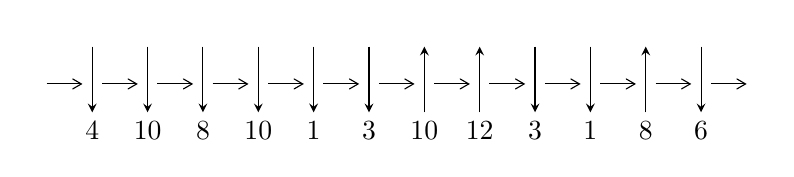
\begin{tikzpicture}[x=20pt, y=17pt]
	% nodes
	\node (C0) at (0, 0) {};
	\node (C1) at (1, 0) {};
	\node (C1U) at (1, +1) {};
	\node (C1D) at (1, -1) {4};

	\node (C2) at (2, 0) {};
	\node (C2U) at (2, +1) {};
	\node (C2D) at (2, -1) {10};

	\node (C3) at (3, 0) {};
	\node (C3U) at (3, +1) {};
	\node (C3D) at (3, -1) {8};

	\node (C4) at (4, 0) {};
	\node (C4U) at (4, +1) {};
	\node (C4D) at (4, -1) {10};

	\node (C5) at (5, 0) {};
	\node (C5U) at (5, +1) {};
	\node (C5D) at (5, -1) {1};

	\node (C6) at (6, 0) {};
	\node (C6U) at (6, +1) {};
	\node (C6D) at (6, -1) {3};

	\node (C7) at (7, 0) {};
	\node (C7U) at (7, +1) {};
	\node (C7D) at (7, -1) {10};

	\node (C8) at (8, 0) {};
	\node (C8U) at (8, +1) {};
	\node (C8D) at (8, -1) {12};

	\node (C9) at (9, 0) {};
	\node (C9U) at (9, +1) {};
	\node (C9D) at (9, -1) {3};

	\node (C10) at (10, 0) {};
	\node (C10U) at (10, +1) {};
	\node (C10D) at (10, -1) {1};

	\node (C11) at (11, 0) {};
	\node (C11U) at (11, +1) {};
	\node (C11D) at (11, -1) {8};

	\node (C12) at (12, 0) {};
	\node (C12U) at (12, +1) {};
	\node (C12D) at (12, -1) {6};
	\node (C13) at (13, 0) {};

	% arrows
	\draw[->,>={angle 60}]
	(C0) edge (C1) (C1) edge (C2) (C2) edge (C3) (C3) edge (C4) (C4) edge (C5) (C5) edge (C6) (C6) edge (C7) (C7) edge (C8) (C8) edge (C9) (C9) edge (C10) (C10) edge (C11) (C11) edge (C12) (C12) edge (C13) ;	\draw[->,>=stealth]
	(C1U) edge (C1D) (C2U) edge (C2D) (C3U) edge (C3D) (C4U) edge (C4D) (C5U) edge (C5D) (C6U) edge (C6D) (C7D) edge (C7U) (C8D) edge (C8U) (C9U) edge (C9D) (C10U) edge (C10D) (C11D) edge (C11U) (C12U) edge (C12D) ;
	\end{tikzpicture} \\
\hhline{~~} \\& 
\textbf{Solving Sequence} \\ \cline{2-2} 
 &
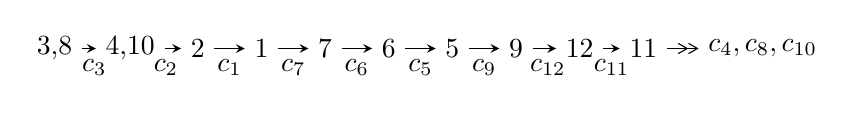
\begin{tikzpicture}[x=23pt, y=7pt]
	% node
	\node (A0) at (-1/8, 0) {3,8};
	\node (A1) at (17/16, 0) {4,10};
	\node (A2) at (17/8, 0) {2};
	\node (A3) at (25/8, 0) {1};
	\node (A4) at (33/8, 0) {7};
	\node (A5) at (41/8, 0) {6};
	\node (A6) at (49/8, 0) {5};
	\node (A7) at (57/8, 0) {9};
	\node (A8) at (65/8, 0) {12};
	\node (A9) at (73/8, 0) {11};
	\node (C1) at (1/2, -1) {$c_{3}$};
	\node (C2) at (13/8, -1) {$c_{2}$};
	\node (C3) at (21/8, -1) {$c_{1}$};
	\node (C4) at (29/8, -1) {$c_{7}$};
	\node (C5) at (37/8, -1) {$c_{6}$};
	\node (C6) at (45/8, -1) {$c_{5}$};
	\node (C7) at (53/8, -1) {$c_{9}$};
	\node (C8) at (61/8, -1) {$c_{12}$};
	\node (C9) at (69/8, -1) {$c_{11}$};
	\node (A10) at (11, 0) {$c_{4},c_{8},c_{10}$};

	% edge
	\draw[->,>=stealth]	
	(A0) edge (A1) (A1) edge (A2) (A2) edge (A3) (A3) edge (A4) (A4) edge (A5) (A5) edge (A6) (A6) edge (A7) (A7) edge (A8) (A8) edge (A9) ;
	\draw[->>,>={angle 60}]	
	(A9) edge (A10);
\end{tikzpicture} \\ 

\end{tabular} \\

\footnotetext{
The image of knot diagram is generated by the software ``\textbf{Draw programme}" developed by Andrew Bartholomew(\url{http://www.layer8.co.uk/maths/draw/index.htm\#Running-draw}), where we modified some parts for our purpose(\url{https://github.com/CATsTAILs/LinksPainter}).
}\phantom \\ \newline 
\centering \textbf{Ideals for irreducible components\footnotemark of $X_{\text{par}}$} 
 
\begin{align*}
I^u_{1}&=\langle 
1.44280\times10^{94} u^{39}+8.50468\times10^{94} u^{38}+\cdots+1.31536\times10^{97} b-5.65969\times10^{97},\\
\phantom{I^u_{1}}&\phantom{= \langle  }-7.99853\times10^{97} u^{39}-1.12262\times10^{98} u^{38}+\cdots+2.19271\times10^{100} a-2.21181\times10^{101},\\
\phantom{I^u_{1}}&\phantom{= \langle  }u^{40}+3 u^{39}+\cdots+1016 u-1667\rangle \\
I^u_{2}&=\langle 
-7910373 u^{16}+432236197 u^{15}+\cdots+1605075802 b+422623648,\\
\phantom{I^u_{2}}&\phantom{= \langle  }996003064 u^{16}-1757434994 u^{15}+\cdots+1605075802 a+2036147287,\;u^{17}-2 u^{16}+\cdots- u^2+1\rangle \\
\\
\end{align*}
\raggedright * 2 irreducible components of $\dim_{\mathbb{C}}=0$, with total 57 representations.\\
\footnotetext{All coefficients of polynomials are rational numbers. But the coefficients are sometimes approximated in decimal forms when there is not enough margin.}
\newpage
\renewcommand{\arraystretch}{1}
\centering \section*{I. $I^u_{1}= \langle 1.44\times10^{94} u^{39}+8.50\times10^{94} u^{38}+\cdots+1.32\times10^{97} b-5.66\times10^{97},\;-8.00\times10^{97} u^{39}-1.12\times10^{98} u^{38}+\cdots+2.19\times10^{100} a-2.21\times10^{101},\;u^{40}+3 u^{39}+\cdots+1016 u-1667 \rangle$}
\flushleft \textbf{(i) Arc colorings}\\
\begin{tabular}{m{7pt} m{180pt} m{7pt} m{180pt} }
\flushright $a_{3}=$&$\begin{pmatrix}1\\0\end{pmatrix}$ \\
\flushright $a_{8}=$&$\begin{pmatrix}0\\u\end{pmatrix}$ \\
\flushright $a_{4}=$&$\begin{pmatrix}1\\u^2\end{pmatrix}$ \\
\flushright $a_{10}=$&$\begin{pmatrix}0.00364778 u^{39}+0.00511977 u^{38}+\cdots-16.1044 u+10.0871\\-0.00109689 u^{39}-0.00646565 u^{38}+\cdots+1.45140 u+4.30276\end{pmatrix}$ \\
\flushright $a_{2}=$&$\begin{pmatrix}-0.00182775 u^{39}+0.0000852465 u^{38}+\cdots+7.45312 u-9.20414\\0.00494909 u^{39}+0.0143198 u^{38}+\cdots-7.75640 u+2.00982\end{pmatrix}$ \\
\flushright $a_{1}=$&$\begin{pmatrix}0.000306195 u^{39}+0.0113462 u^{38}+\cdots+8.40116 u-16.4770\\0.00369323 u^{39}+0.00540172 u^{38}+\cdots-9.13598 u+10.1100\end{pmatrix}$ \\
\flushright $a_{7}=$&$\begin{pmatrix}-0.0149546 u^{39}-0.0418621 u^{38}+\cdots+30.1162 u-7.15726\\0.00556849 u^{39}+0.0195206 u^{38}+\cdots-7.34714 u-3.04686\end{pmatrix}$ \\
\flushright $a_{6}=$&$\begin{pmatrix}-0.00938611 u^{39}-0.0223414 u^{38}+\cdots+22.7690 u-10.2041\\0.00556849 u^{39}+0.0195206 u^{38}+\cdots-7.34714 u-3.04686\end{pmatrix}$ \\
\flushright $a_{5}=$&$\begin{pmatrix}0.00482950 u^{39}+0.0248160 u^{38}+\cdots+0.583500 u-13.7252\\-0.00213394 u^{39}-0.0112609 u^{38}+\cdots-0.948044 u+7.27286\end{pmatrix}$ \\
\flushright $a_{9}=$&$\begin{pmatrix}0.00255090 u^{39}-0.00134588 u^{38}+\cdots-14.6530 u+14.3899\\-0.00109689 u^{39}-0.00646565 u^{38}+\cdots+1.45140 u+4.30276\end{pmatrix}$ \\
\flushright $a_{12}=$&$\begin{pmatrix}-0.00391056 u^{39}-0.0175058 u^{38}+\cdots+6.93355 u+8.56793\\-0.00163120 u^{39}-0.00313351 u^{38}+\cdots+5.54321 u-3.60264\end{pmatrix}$ \\
\flushright $a_{11}=$&$\begin{pmatrix}-0.00391056 u^{39}-0.0175058 u^{38}+\cdots+6.93355 u+8.56793\\0.00128477 u^{39}+0.0119254 u^{38}+\cdots+4.89087 u-13.2282\end{pmatrix}$\\&\end{tabular}
\flushleft \textbf{(ii) Obstruction class $= -1$}\\~\\
\flushleft \textbf{(iii) Cusp Shapes $= 0.0225460 u^{39}+0.0929089 u^{38}+\cdots+1.19705 u-39.3928$}\\~\\
\newpage\renewcommand{\arraystretch}{1}
\flushleft \textbf{(iv) u-Polynomials at the component}\newline \\
\begin{tabular}{m{50pt}|m{274pt}}
Crossings & \hspace{64pt}u-Polynomials at each crossing \\
\hline $$\begin{aligned}c_{1}\end{aligned}$$&$\begin{aligned}
&u^{40}-6 u^{39}+\cdots-585 u+81
\end{aligned}$\\
\hline $$\begin{aligned}c_{2},c_{9}\end{aligned}$$&$\begin{aligned}
&u^{40}+u^{39}+\cdots-1593 u-281
\end{aligned}$\\
\hline $$\begin{aligned}c_{3}\end{aligned}$$&$\begin{aligned}
&u^{40}-3 u^{39}+\cdots-1016 u-1667
\end{aligned}$\\
\hline $$\begin{aligned}c_{4}\end{aligned}$$&$\begin{aligned}
&u^{40}-2 u^{39}+\cdots+18 u-7
\end{aligned}$\\
\hline $$\begin{aligned}c_{5},c_{12}\end{aligned}$$&$\begin{aligned}
&u^{40}+2 u^{39}+\cdots+45 u-181
\end{aligned}$\\
\hline $$\begin{aligned}c_{6}\end{aligned}$$&$\begin{aligned}
&u^{40}+23 u^{38}+\cdots+72246 u-10339
\end{aligned}$\\
\hline $$\begin{aligned}c_{7}\end{aligned}$$&$\begin{aligned}
&u^{40}- u^{39}+\cdots+119 u+7
\end{aligned}$\\
\hline $$\begin{aligned}c_{8},c_{11}\end{aligned}$$&$\begin{aligned}
&u^{40}-4 u^{39}+\cdots+159 u+39
\end{aligned}$\\
\hline $$\begin{aligned}c_{10}\end{aligned}$$&$\begin{aligned}
&u^{40}-3 u^{39}+\cdots+77 u+49
\end{aligned}$\\
\hline
\end{tabular}\\~\\
\newpage\renewcommand{\arraystretch}{1}
\flushleft \textbf{(v) Riley Polynomials at the component}\newline \\
\begin{tabular}{m{50pt}|m{274pt}}
Crossings & \hspace{64pt}Riley Polynomials at each crossing \\
\hline $$\begin{aligned}c_{1}\end{aligned}$$&$\begin{aligned}
&y^{40}-22 y^{39}+\cdots-215217 y+6561
\end{aligned}$\\
\hline $$\begin{aligned}c_{2},c_{9}\end{aligned}$$&$\begin{aligned}
&y^{40}+55 y^{39}+\cdots+1314861 y+78961
\end{aligned}$\\
\hline $$\begin{aligned}c_{3}\end{aligned}$$&$\begin{aligned}
&y^{40}+35 y^{39}+\cdots+25863122 y+2778889
\end{aligned}$\\
\hline $$\begin{aligned}c_{4}\end{aligned}$$&$\begin{aligned}
&y^{40}-38 y^{39}+\cdots+10176 y+49
\end{aligned}$\\
\hline $$\begin{aligned}c_{5},c_{12}\end{aligned}$$&$\begin{aligned}
&y^{40}+28 y^{39}+\cdots+424773 y+32761
\end{aligned}$\\
\hline $$\begin{aligned}c_{6}\end{aligned}$$&$\begin{aligned}
&y^{40}+46 y^{39}+\cdots-3212684616 y+106894921
\end{aligned}$\\
\hline $$\begin{aligned}c_{7}\end{aligned}$$&$\begin{aligned}
&y^{40}-55 y^{39}+\cdots-3745 y+49
\end{aligned}$\\
\hline $$\begin{aligned}c_{8},c_{11}\end{aligned}$$&$\begin{aligned}
&y^{40}-22 y^{39}+\cdots-88383 y+1521
\end{aligned}$\\
\hline $$\begin{aligned}c_{10}\end{aligned}$$&$\begin{aligned}
&y^{40}-29 y^{39}+\cdots-130291 y+2401
\end{aligned}$\\
\hline
\end{tabular}\\~\\
\newpage\flushleft \textbf{(vi) Complex Volumes and Cusp Shapes}
$$\begin{array}{c|c|c}  
\text{Solutions to }I^u_{1}& \I (\text{vol} + \sqrt{-1}CS) & \text{Cusp shape}\\
 \hline 
\begin{aligned}
u &= \phantom{-}0.074225 + 0.995798 I \\
a &= -1.48142 - 0.88202 I \\
b &= \phantom{-}0.069778 + 0.251836 I\end{aligned}
 & -1.68029 - 6.30373 I & -1.75666 + 6.49211 I \\ \hline\begin{aligned}
u &= \phantom{-}0.074225 - 0.995798 I \\
a &= -1.48142 + 0.88202 I \\
b &= \phantom{-}0.069778 - 0.251836 I\end{aligned}
 & -1.68029 + 6.30373 I & -1.75666 - 6.49211 I \\ \hline\begin{aligned}
u &= -0.019908 + 1.014730 I \\
a &= \phantom{-}0.933442 + 0.125283 I \\
b &= \phantom{-}0.321710 + 0.172172 I\end{aligned}
 & -2.72752 - 0.30261 I & -4.74009 + 1.12705 I \\ \hline\begin{aligned}
u &= -0.019908 - 1.014730 I \\
a &= \phantom{-}0.933442 - 0.125283 I \\
b &= \phantom{-}0.321710 - 0.172172 I\end{aligned}
 & -2.72752 + 0.30261 I & -4.74009 - 1.12705 I \\ \hline\begin{aligned}
u &= \phantom{-}0.090932 + 1.056100 I \\
a &= \phantom{-}0.69809 - 1.51032 I \\
b &= \phantom{-}0.39797 + 1.53949 I\end{aligned}
 & \phantom{-}8.40378 + 2.27498 I & -2.47436 - 4.06313 I \\ \hline\begin{aligned}
u &= \phantom{-}0.090932 - 1.056100 I \\
a &= \phantom{-}0.69809 + 1.51032 I \\
b &= \phantom{-}0.39797 - 1.53949 I\end{aligned}
 & \phantom{-}8.40378 - 2.27498 I & -2.47436 + 4.06313 I \\ \hline\begin{aligned}
u &= -0.384077 + 0.999119 I \\
a &= -0.75184 - 1.68276 I \\
b &= -0.06076 + 1.71893 I\end{aligned}
 & \phantom{-}9.33802 - 0.43323 I & -1.80383 - 1.69832 I \\ \hline\begin{aligned}
u &= -0.384077 - 0.999119 I \\
a &= -0.75184 + 1.68276 I \\
b &= -0.06076 - 1.71893 I\end{aligned}
 & \phantom{-}9.33802 + 0.43323 I & -1.80383 + 1.69832 I \\ \hline\begin{aligned}
u &= \phantom{-}0.744898 + 0.775177 I \\
a &= -0.209036 - 0.214334 I \\
b &= -1.145770 + 0.121712 I\end{aligned}
 & -4.62154 - 2.17421 I & -9.73588 + 5.09039 I \\ \hline\begin{aligned}
u &= \phantom{-}0.744898 - 0.775177 I \\
a &= -0.209036 + 0.214334 I \\
b &= -1.145770 - 0.121712 I\end{aligned}
 & -4.62154 + 2.17421 I & -9.73588 - 5.09039 I\\
 \hline 
 \end{array}$$\newpage$$\begin{array}{c|c|c}  
\text{Solutions to }I^u_{1}& \I (\text{vol} + \sqrt{-1}CS) & \text{Cusp shape}\\
 \hline 
\begin{aligned}
u &= \phantom{-}0.969293 + 0.598574 I \\
a &= \phantom{-}0.875542 - 0.894161 I \\
b &= -0.124340 + 0.752925 I\end{aligned}
 & -0.244335 - 1.176990 I & -6.16007 + 1.36199 I \\ \hline\begin{aligned}
u &= \phantom{-}0.969293 - 0.598574 I \\
a &= \phantom{-}0.875542 + 0.894161 I \\
b &= -0.124340 - 0.752925 I\end{aligned}
 & -0.244335 + 1.176990 I & -6.16007 - 1.36199 I \\ \hline\begin{aligned}
u &= -1.103180 + 0.358015 I \\
a &= \phantom{-}0.751248 + 0.156995 I \\
b &= \phantom{-}0.530673 - 0.765497 I\end{aligned}
 & -1.66991 + 2.90598 I & -0.37953 - 2.28494 I \\ \hline\begin{aligned}
u &= -1.103180 - 0.358015 I \\
a &= \phantom{-}0.751248 - 0.156995 I \\
b &= \phantom{-}0.530673 + 0.765497 I\end{aligned}
 & -1.66991 - 2.90598 I & -0.37953 + 2.28494 I \\ \hline\begin{aligned}
u &= -0.898417 + 0.778153 I \\
a &= \phantom{-}0.096570 - 0.403680 I \\
b &= -0.535046 - 0.126132 I\end{aligned}
 & \phantom{-}4.45088 + 3.00898 I & -9.22623 + 0.17791 I \\ \hline\begin{aligned}
u &= -0.898417 - 0.778153 I \\
a &= \phantom{-}0.096570 + 0.403680 I \\
b &= -0.535046 + 0.126132 I\end{aligned}
 & \phantom{-}4.45088 - 3.00898 I & -9.22623 - 0.17791 I \\ \hline\begin{aligned}
u &= \phantom{-}0.530454 + 1.115730 I \\
a &= -0.109870 + 0.125763 I \\
b &= \phantom{-}1.69402 - 0.58477 I\end{aligned}
 & -1.60625 + 4.02862 I & -2.67808 - 1.97162 I \\ \hline\begin{aligned}
u &= \phantom{-}0.530454 - 1.115730 I \\
a &= -0.109870 - 0.125763 I \\
b &= \phantom{-}1.69402 + 0.58477 I\end{aligned}
 & -1.60625 - 4.02862 I & -2.67808 + 1.97162 I \\ \hline\begin{aligned}
u &= \phantom{-}0.946367 + 0.805651 I \\
a &= -0.594098 + 0.206972 I \\
b &= \phantom{-}0.866066 - 0.936600 I\end{aligned}
 & \phantom{-}0.05822 - 3.02351 I & -2.19172 + 2.97004 I \\ \hline\begin{aligned}
u &= \phantom{-}0.946367 - 0.805651 I \\
a &= -0.594098 - 0.206972 I \\
b &= \phantom{-}0.866066 + 0.936600 I\end{aligned}
 & \phantom{-}0.05822 + 3.02351 I & -2.19172 - 2.97004 I\\
 \hline 
 \end{array}$$\newpage$$\begin{array}{c|c|c}  
\text{Solutions to }I^u_{1}& \I (\text{vol} + \sqrt{-1}CS) & \text{Cusp shape}\\
 \hline 
\begin{aligned}
u &= \phantom{-}0.547294 + 1.146790 I \\
a &= \phantom{-}0.07437 - 1.44792 I \\
b &= \phantom{-}0.351725 + 1.262160 I\end{aligned}
 & \phantom{-}1.36525 - 2.63988 I & \phantom{-}0.758920 - 0.234307 I \\ \hline\begin{aligned}
u &= \phantom{-}0.547294 - 1.146790 I \\
a &= \phantom{-}0.07437 + 1.44792 I \\
b &= \phantom{-}0.351725 - 1.262160 I\end{aligned}
 & \phantom{-}1.36525 + 2.63988 I & \phantom{-}0.758920 + 0.234307 I \\ \hline\begin{aligned}
u &= \phantom{-}0.110521 + 1.325330 I \\
a &= -0.210888 + 1.057420 I \\
b &= -0.82951 - 1.82120 I\end{aligned}
 & \phantom{-}9.68403 - 3.29803 I & -1.76650 + 2.63916 I \\ \hline\begin{aligned}
u &= \phantom{-}0.110521 - 1.325330 I \\
a &= -0.210888 - 1.057420 I \\
b &= -0.82951 + 1.82120 I\end{aligned}
 & \phantom{-}9.68403 + 3.29803 I & -1.76650 - 2.63916 I \\ \hline\begin{aligned}
u &= -0.400029 + 1.319180 I \\
a &= \phantom{-}0.302273 + 1.229320 I \\
b &= \phantom{-}0.25236 - 2.15666 I\end{aligned}
 & \phantom{-}10.73370 + 3.93558 I & -1.98176 - 4.05917 I \\ \hline\begin{aligned}
u &= -0.400029 - 1.319180 I \\
a &= \phantom{-}0.302273 - 1.229320 I \\
b &= \phantom{-}0.25236 + 2.15666 I\end{aligned}
 & \phantom{-}10.73370 - 3.93558 I & -1.98176 + 4.05917 I \\ \hline\begin{aligned}
u &= \phantom{-}0.499216\phantom{ +0.000000I} \\
a &= -0.294586\phantom{ +0.000000I} \\
b &= \phantom{-}0.384818\phantom{ +0.000000I}\end{aligned}
 & -0.791835\phantom{ +0.000000I} & -13.1510\phantom{ +0.000000I} \\ \hline\begin{aligned}
u &= \phantom{-}0.60667 + 1.39679 I \\
a &= -0.177788 + 1.087880 I \\
b &= \phantom{-}0.08306 - 1.87544 I\end{aligned}
 & \phantom{-}2.61258 - 4.98918 I & \phantom{-0.000000 } 0 \\ \hline\begin{aligned}
u &= \phantom{-}0.60667 - 1.39679 I \\
a &= -0.177788 - 1.087880 I \\
b &= \phantom{-}0.08306 + 1.87544 I\end{aligned}
 & \phantom{-}2.61258 + 4.98918 I & \phantom{-0.000000 } 0 \\ \hline\begin{aligned}
u &= \phantom{-}0.057521 + 0.459196 I \\
a &= -1.04344 - 1.83286 I \\
b &= -0.049531 + 0.594009 I\end{aligned}
 & \phantom{-}1.36870 - 1.27202 I & \phantom{-}0.60073 + 4.17984 I\\
 \hline 
 \end{array}$$\newpage$$\begin{array}{c|c|c}  
\text{Solutions to }I^u_{1}& \I (\text{vol} + \sqrt{-1}CS) & \text{Cusp shape}\\
 \hline 
\begin{aligned}
u &= \phantom{-}0.057521 - 0.459196 I \\
a &= -1.04344 + 1.83286 I \\
b &= -0.049531 - 0.594009 I\end{aligned}
 & \phantom{-}1.36870 + 1.27202 I & \phantom{-}0.60073 - 4.17984 I \\ \hline\begin{aligned}
u &= -0.451499\phantom{ +0.000000I} \\
a &= \phantom{-}1.24714\phantom{ +0.000000I} \\
b &= -1.34904\phantom{ +0.000000I}\end{aligned}
 & -7.99269\phantom{ +0.000000I} & -41.4500\phantom{ +0.000000I} \\ \hline\begin{aligned}
u &= -1.71262 + 0.03239 I \\
a &= -0.625667 - 0.062971 I \\
b &= -0.701464 + 1.129030 I\end{aligned}
 & \phantom{-}2.55596 - 3.89352 I & \phantom{-0.000000 } 0 \\ \hline\begin{aligned}
u &= -1.71262 - 0.03239 I \\
a &= -0.625667 + 0.062971 I \\
b &= -0.701464 - 1.129030 I\end{aligned}
 & \phantom{-}2.55596 + 3.89352 I & \phantom{-0.000000 } 0 \\ \hline\begin{aligned}
u &= -0.93976 + 1.68582 I \\
a &= \phantom{-}0.302089 + 0.934011 I \\
b &= \phantom{-}0.52563 - 2.12471 I\end{aligned}
 & \phantom{-}7.2434 + 13.4515 I & \phantom{-0.000000 } 0 \\ \hline\begin{aligned}
u &= -0.93976 - 1.68582 I \\
a &= \phantom{-}0.302089 - 0.934011 I \\
b &= \phantom{-}0.52563 + 2.12471 I\end{aligned}
 & \phantom{-}7.2434 - 13.4515 I & \phantom{-0.000000 } 0 \\ \hline\begin{aligned}
u &= -0.75189 + 1.95033 I \\
a &= -0.179356 - 0.815834 I \\
b &= -0.24537 + 2.12821 I\end{aligned}
 & \phantom{-}4.31816 + 4.85736 I & \phantom{-0.000000 } 0 \\ \hline\begin{aligned}
u &= -0.75189 - 1.95033 I \\
a &= -0.179356 + 0.815834 I \\
b &= -0.24537 - 2.12821 I\end{aligned}
 & \phantom{-}4.31816 - 4.85736 I & \phantom{-0.000000 } 0 \\ \hline\begin{aligned}
u &= \phantom{-}0.00784 + 2.54288 I \\
a &= -0.024216 + 0.721328 I \\
b &= -0.41910 - 2.14226 I\end{aligned}
 & \phantom{-}13.20450 - 2.73784 I & \phantom{-0.000000 } 0 \\ \hline\begin{aligned}
u &= \phantom{-}0.00784 - 2.54288 I \\
a &= -0.024216 - 0.721328 I \\
b &= -0.41910 + 2.14226 I\end{aligned}
 & \phantom{-}13.20450 + 2.73784 I & \phantom{-0.000000 } 0\\
 \hline 
 \end{array}$$\newpage\newpage\renewcommand{\arraystretch}{1}
\centering \section*{II. $I^u_{2}= \langle -7.91\times10^{6} u^{16}+4.32\times10^{8} u^{15}+\cdots+1.61\times10^{9} b+4.23\times10^{8},\;9.96\times10^{8} u^{16}-1.76\times10^{9} u^{15}+\cdots+1.61\times10^{9} a+2.04\times10^{9},\;u^{17}-2 u^{16}+\cdots- u^2+1 \rangle$}
\flushleft \textbf{(i) Arc colorings}\\
\begin{tabular}{m{7pt} m{180pt} m{7pt} m{180pt} }
\flushright $a_{3}=$&$\begin{pmatrix}1\\0\end{pmatrix}$ \\
\flushright $a_{8}=$&$\begin{pmatrix}0\\u\end{pmatrix}$ \\
\flushright $a_{4}=$&$\begin{pmatrix}1\\u^2\end{pmatrix}$ \\
\flushright $a_{10}=$&$\begin{pmatrix}-0.620533 u^{16}+1.09492 u^{15}+\cdots-0.305972 u-1.26857\\0.00492835 u^{16}-0.269293 u^{15}+\cdots-1.22753 u-0.263304\end{pmatrix}$ \\
\flushright $a_{2}=$&$\begin{pmatrix}-0.151781 u^{16}+0.152336 u^{15}+\cdots-4.08959 u+0.621432\\-0.149622 u^{16}+0.0695177 u^{15}+\cdots+1.46667 u-1.24998\end{pmatrix}$ \\
\flushright $a_{1}=$&$\begin{pmatrix}-0.498942 u^{16}+0.618046 u^{15}+\cdots-2.77470 u-0.779776\\-0.274767 u^{16}+0.350118 u^{15}+\cdots+1.81383 u-1.02137\end{pmatrix}$ \\
\flushright $a_{7}=$&$\begin{pmatrix}-0.537305 u^{16}+1.17062 u^{15}+\cdots-0.571419 u+2.57166\\-0.151225 u^{16}+0.499990 u^{15}+\cdots+0.621432 u+0.151781\end{pmatrix}$ \\
\flushright $a_{6}=$&$\begin{pmatrix}-0.688530 u^{16}+1.67061 u^{15}+\cdots+0.0500138 u+2.72344\\-0.151225 u^{16}+0.499990 u^{15}+\cdots+0.621432 u+0.151781\end{pmatrix}$ \\
\flushright $a_{5}=$&$\begin{pmatrix}0.247793 u^{16}-0.451462 u^{15}+\cdots+6.66125 u+1.91587\\0.347162 u^{16}-0.465710 u^{15}+\cdots-1.31489 u+1.40121\end{pmatrix}$ \\
\flushright $a_{9}=$&$\begin{pmatrix}-0.615605 u^{16}+0.825630 u^{15}+\cdots-1.53350 u-1.53187\\0.00492835 u^{16}-0.269293 u^{15}+\cdots-1.22753 u-0.263304\end{pmatrix}$ \\
\flushright $a_{12}=$&$\begin{pmatrix}0.606095 u^{16}-1.10067 u^{15}+\cdots+2.24416 u+1.10418\\-0.0253392 u^{16}+0.352876 u^{15}+\cdots+3.62140 u-1.08505\end{pmatrix}$ \\
\flushright $a_{11}=$&$\begin{pmatrix}0.606095 u^{16}-1.10067 u^{15}+\cdots+2.24416 u+1.10418\\-0.171636 u^{16}+0.583572 u^{15}+\cdots+3.01530 u-1.19657\end{pmatrix}$\\&\end{tabular}
\flushleft \textbf{(ii) Obstruction class $= 1$}\\~\\
\flushleft \textbf{(iii) Cusp Shapes $= \frac{7112656685}{1605075802} u^{16}-\frac{7923058150}{802537901} u^{15}+\cdots-\frac{29249964323}{1605075802} u-\frac{13984566}{802537901}$}\\~\\
\newpage\renewcommand{\arraystretch}{1}
\flushleft \textbf{(iv) u-Polynomials at the component}\newline \\
\begin{tabular}{m{50pt}|m{274pt}}
Crossings & \hspace{64pt}u-Polynomials at each crossing \\
\hline $$\begin{aligned}c_{1}\end{aligned}$$&$\begin{aligned}
&u^{17}-7 u^{16}+\cdots+33 u-11
\end{aligned}$\\
\hline $$\begin{aligned}c_{2}\end{aligned}$$&$\begin{aligned}
&u^{17}+6 u^{15}+\cdots-9 u-1
\end{aligned}$\\
\hline $$\begin{aligned}c_{3}\end{aligned}$$&$\begin{aligned}
&u^{17}-2 u^{16}+\cdots- u^2+1
\end{aligned}$\\
\hline $$\begin{aligned}c_{4}\end{aligned}$$&$\begin{aligned}
&u^{17}+u^{16}+\cdots+84 u-19
\end{aligned}$\\
\hline $$\begin{aligned}c_{5}\end{aligned}$$&$\begin{aligned}
&u^{17}- u^{16}+\cdots+u-1
\end{aligned}$\\
\hline $$\begin{aligned}c_{6}\end{aligned}$$&$\begin{aligned}
&u^{17}+u^{16}+\cdots-14 u-1
\end{aligned}$\\
\hline $$\begin{aligned}c_{7}\end{aligned}$$&$\begin{aligned}
&u^{17}+6 u^{16}+\cdots+45 u+11
\end{aligned}$\\
\hline $$\begin{aligned}c_{8}\end{aligned}$$&$\begin{aligned}
&u^{17}-3 u^{16}+\cdots+u-1
\end{aligned}$\\
\hline $$\begin{aligned}c_{9}\end{aligned}$$&$\begin{aligned}
&u^{17}+6 u^{15}+\cdots-9 u+1
\end{aligned}$\\
\hline $$\begin{aligned}c_{10}\end{aligned}$$&$\begin{aligned}
&u^{17}-4 u^{16}+\cdots-5 u-1
\end{aligned}$\\
\hline $$\begin{aligned}c_{11}\end{aligned}$$&$\begin{aligned}
&u^{17}+3 u^{16}+\cdots+u+1
\end{aligned}$\\
\hline $$\begin{aligned}c_{12}\end{aligned}$$&$\begin{aligned}
&u^{17}+u^{16}+\cdots+u+1
\end{aligned}$\\
\hline
\end{tabular}\\~\\
\newpage\renewcommand{\arraystretch}{1}
\flushleft \textbf{(v) Riley Polynomials at the component}\newline \\
\begin{tabular}{m{50pt}|m{274pt}}
Crossings & \hspace{64pt}Riley Polynomials at each crossing \\
\hline $$\begin{aligned}c_{1}\end{aligned}$$&$\begin{aligned}
&y^{17}-13 y^{16}+\cdots+561 y-121
\end{aligned}$\\
\hline $$\begin{aligned}c_{2},c_{9}\end{aligned}$$&$\begin{aligned}
&y^{17}+12 y^{16}+\cdots+19 y-1
\end{aligned}$\\
\hline $$\begin{aligned}c_{3}\end{aligned}$$&$\begin{aligned}
&y^{17}+12 y^{16}+\cdots+2 y-1
\end{aligned}$\\
\hline $$\begin{aligned}c_{4}\end{aligned}$$&$\begin{aligned}
&y^{17}-13 y^{16}+\cdots+3104 y-361
\end{aligned}$\\
\hline $$\begin{aligned}c_{5},c_{12}\end{aligned}$$&$\begin{aligned}
&y^{17}+9 y^{16}+\cdots+11 y-1
\end{aligned}$\\
\hline $$\begin{aligned}c_{6}\end{aligned}$$&$\begin{aligned}
&y^{17}+11 y^{16}+\cdots+72 y-1
\end{aligned}$\\
\hline $$\begin{aligned}c_{7}\end{aligned}$$&$\begin{aligned}
&y^{17}-22 y^{16}+\cdots+1321 y-121
\end{aligned}$\\
\hline $$\begin{aligned}c_{8},c_{11}\end{aligned}$$&$\begin{aligned}
&y^{17}-9 y^{16}+\cdots+7 y-1
\end{aligned}$\\
\hline $$\begin{aligned}c_{10}\end{aligned}$$&$\begin{aligned}
&y^{17}-12 y^{16}+\cdots+11 y-1
\end{aligned}$\\
\hline
\end{tabular}\\~\\
\newpage\flushleft \textbf{(vi) Complex Volumes and Cusp Shapes}
$$\begin{array}{c|c|c}  
\text{Solutions to }I^u_{2}& \I (\text{vol} + \sqrt{-1}CS) & \text{Cusp shape}\\
 \hline 
\begin{aligned}
u &= \phantom{-}0.020499 + 0.998308 I \\
a &= \phantom{-}0.37175 - 1.89988 I \\
b &= \phantom{-}0.18081 + 1.72832 I\end{aligned}
 & \phantom{-}9.62563 + 1.51829 I & \phantom{-}1.39343 - 3.45515 I \\ \hline\begin{aligned}
u &= \phantom{-}0.020499 - 0.998308 I \\
a &= \phantom{-}0.37175 + 1.89988 I \\
b &= \phantom{-}0.18081 - 1.72832 I\end{aligned}
 & \phantom{-}9.62563 - 1.51829 I & \phantom{-}1.39343 + 3.45515 I \\ \hline\begin{aligned}
u &= -0.380557 + 0.938672 I \\
a &= \phantom{-}0.739410 + 0.323312 I \\
b &= \phantom{-}1.246230 - 0.332058 I\end{aligned}
 & -4.22062 + 1.12566 I & -5.94166 + 0.72076 I \\ \hline\begin{aligned}
u &= -0.380557 - 0.938672 I \\
a &= \phantom{-}0.739410 - 0.323312 I \\
b &= \phantom{-}1.246230 + 0.332058 I\end{aligned}
 & -4.22062 - 1.12566 I & -5.94166 - 0.72076 I \\ \hline\begin{aligned}
u &= -0.995936 + 0.621165 I \\
a &= -0.280702 - 0.424421 I \\
b &= -0.353305 - 0.553264 I\end{aligned}
 & \phantom{-}5.01697 + 3.35175 I & \phantom{-}1.60696 - 5.55747 I \\ \hline\begin{aligned}
u &= -0.995936 - 0.621165 I \\
a &= -0.280702 + 0.424421 I \\
b &= -0.353305 + 0.553264 I\end{aligned}
 & \phantom{-}5.01697 - 3.35175 I & \phantom{-}1.60696 + 5.55747 I \\ \hline\begin{aligned}
u &= \phantom{-}1.178520 + 0.479735 I \\
a &= -0.655660 + 0.253208 I \\
b &= -0.090891 - 0.717128 I\end{aligned}
 & -2.58072 - 3.16432 I & -9.05012 + 4.68936 I \\ \hline\begin{aligned}
u &= \phantom{-}1.178520 - 0.479735 I \\
a &= -0.655660 - 0.253208 I \\
b &= -0.090891 + 0.717128 I\end{aligned}
 & -2.58072 + 3.16432 I & -9.05012 - 4.68936 I \\ \hline\begin{aligned}
u &= \phantom{-}0.692730 + 0.052899 I \\
a &= \phantom{-}1.72978 + 0.41261 I \\
b &= -0.232122 - 0.090819 I\end{aligned}
 & \phantom{-}0.745228 + 0.220813 I & -1.69301 + 1.79583 I \\ \hline\begin{aligned}
u &= \phantom{-}0.692730 - 0.052899 I \\
a &= \phantom{-}1.72978 - 0.41261 I \\
b &= -0.232122 + 0.090819 I\end{aligned}
 & \phantom{-}0.745228 - 0.220813 I & -1.69301 - 1.79583 I\\
 \hline 
 \end{array}$$\newpage$$\begin{array}{c|c|c}  
\text{Solutions to }I^u_{2}& \I (\text{vol} + \sqrt{-1}CS) & \text{Cusp shape}\\
 \hline 
\begin{aligned}
u &= \phantom{-}0.531547 + 1.299730 I \\
a &= \phantom{-}0.013837 - 1.218520 I \\
b &= \phantom{-}0.113827 + 1.336070 I\end{aligned}
 & \phantom{-}0.72305 - 3.21935 I & -6.16546 + 5.06885 I \\ \hline\begin{aligned}
u &= \phantom{-}0.531547 - 1.299730 I \\
a &= \phantom{-}0.013837 + 1.218520 I \\
b &= \phantom{-}0.113827 - 1.336070 I\end{aligned}
 & \phantom{-}0.72305 + 3.21935 I & -6.16546 - 5.06885 I \\ \hline\begin{aligned}
u &= \phantom{-}0.016024 + 0.519282 I \\
a &= -1.90689 - 1.51776 I \\
b &= -1.092870 + 0.142474 I\end{aligned}
 & -2.88743 - 5.63292 I & -6.98267 + 4.20336 I \\ \hline\begin{aligned}
u &= \phantom{-}0.016024 - 0.519282 I \\
a &= -1.90689 + 1.51776 I \\
b &= -1.092870 - 0.142474 I\end{aligned}
 & -2.88743 + 5.63292 I & -6.98267 - 4.20336 I \\ \hline\begin{aligned}
u &= -0.346914\phantom{ +0.000000I} \\
a &= -1.87486\phantom{ +0.000000I} \\
b &= \phantom{-}1.39658\phantom{ +0.000000I}\end{aligned}
 & -7.87029\phantom{ +0.000000I} & \phantom{-}24.2710\phantom{ +0.000000I} \\ \hline\begin{aligned}
u &= \phantom{-}0.11063 + 2.21488 I \\
a &= -0.074096 + 0.817459 I \\
b &= -0.46997 - 2.10827 I\end{aligned}
 & \phantom{-}13.9624 - 2.5342 I & \phantom{-}2.69679 + 0.52341 I \\ \hline\begin{aligned}
u &= \phantom{-}0.11063 - 2.21488 I \\
a &= -0.074096 - 0.817459 I \\
b &= -0.46997 + 2.10827 I\end{aligned}
 & \phantom{-}13.9624 + 2.5342 I & \phantom{-}2.69679 - 0.52341 I\\
 \hline 
 \end{array}$$\newpage
\newpage\renewcommand{\arraystretch}{1}
\centering \section*{ III. u-Polynomials}
\begin{tabular}{m{50pt}|m{274pt}}
Crossings & \hspace{64pt}u-Polynomials at each crossing \\
\hline $$\begin{aligned}c_{1}\end{aligned}$$&$\begin{aligned}
&(u^{17}-7 u^{16}+\cdots+33 u-11)(u^{40}-6 u^{39}+\cdots-585 u+81)
\end{aligned}$\\
\hline $$\begin{aligned}c_{2}\end{aligned}$$&$\begin{aligned}
&(u^{17}+6 u^{15}+\cdots-9 u-1)(u^{40}+u^{39}+\cdots-1593 u-281)
\end{aligned}$\\
\hline $$\begin{aligned}c_{3}\end{aligned}$$&$\begin{aligned}
&(u^{17}-2 u^{16}+\cdots- u^2+1)(u^{40}-3 u^{39}+\cdots-1016 u-1667)
\end{aligned}$\\
\hline $$\begin{aligned}c_{4}\end{aligned}$$&$\begin{aligned}
&(u^{17}+u^{16}+\cdots+84 u-19)(u^{40}-2 u^{39}+\cdots+18 u-7)
\end{aligned}$\\
\hline $$\begin{aligned}c_{5}\end{aligned}$$&$\begin{aligned}
&(u^{17}- u^{16}+\cdots+u-1)(u^{40}+2 u^{39}+\cdots+45 u-181)
\end{aligned}$\\
\hline $$\begin{aligned}c_{6}\end{aligned}$$&$\begin{aligned}
&(u^{17}+u^{16}+\cdots-14 u-1)(u^{40}+23 u^{38}+\cdots+72246 u-10339)
\end{aligned}$\\
\hline $$\begin{aligned}c_{7}\end{aligned}$$&$\begin{aligned}
&(u^{17}+6 u^{16}+\cdots+45 u+11)(u^{40}- u^{39}+\cdots+119 u+7)
\end{aligned}$\\
\hline $$\begin{aligned}c_{8}\end{aligned}$$&$\begin{aligned}
&(u^{17}-3 u^{16}+\cdots+u-1)(u^{40}-4 u^{39}+\cdots+159 u+39)
\end{aligned}$\\
\hline $$\begin{aligned}c_{9}\end{aligned}$$&$\begin{aligned}
&(u^{17}+6 u^{15}+\cdots-9 u+1)(u^{40}+u^{39}+\cdots-1593 u-281)
\end{aligned}$\\
\hline $$\begin{aligned}c_{10}\end{aligned}$$&$\begin{aligned}
&(u^{17}-4 u^{16}+\cdots-5 u-1)(u^{40}-3 u^{39}+\cdots+77 u+49)
\end{aligned}$\\
\hline $$\begin{aligned}c_{11}\end{aligned}$$&$\begin{aligned}
&(u^{17}+3 u^{16}+\cdots+u+1)(u^{40}-4 u^{39}+\cdots+159 u+39)
\end{aligned}$\\
\hline $$\begin{aligned}c_{12}\end{aligned}$$&$\begin{aligned}
&(u^{17}+u^{16}+\cdots+u+1)(u^{40}+2 u^{39}+\cdots+45 u-181)
\end{aligned}$\\
\hline
\end{tabular}\newpage\renewcommand{\arraystretch}{1}
\centering \section*{ IV. Riley Polynomials}
\begin{tabular}{m{50pt}|m{274pt}}
Crossings & \hspace{64pt}Riley Polynomials at each crossing \\
\hline $$\begin{aligned}c_{1}\end{aligned}$$&$\begin{aligned}
&(y^{17}-13 y^{16}+\cdots+561 y-121)\\
&\cdot(y^{40}-22 y^{39}+\cdots-215217 y+6561)
\end{aligned}$\\
\hline $$\begin{aligned}c_{2},c_{9}\end{aligned}$$&$\begin{aligned}
&(y^{17}+12 y^{16}+\cdots+19 y-1)(y^{40}+55 y^{39}+\cdots+1314861 y+78961)
\end{aligned}$\\
\hline $$\begin{aligned}c_{3}\end{aligned}$$&$\begin{aligned}
&(y^{17}+12 y^{16}+\cdots+2 y-1)\\
&\cdot(y^{40}+35 y^{39}+\cdots+25863122 y+2778889)
\end{aligned}$\\
\hline $$\begin{aligned}c_{4}\end{aligned}$$&$\begin{aligned}
&(y^{17}-13 y^{16}+\cdots+3104 y-361)(y^{40}-38 y^{39}+\cdots+10176 y+49)
\end{aligned}$\\
\hline $$\begin{aligned}c_{5},c_{12}\end{aligned}$$&$\begin{aligned}
&(y^{17}+9 y^{16}+\cdots+11 y-1)(y^{40}+28 y^{39}+\cdots+424773 y+32761)
\end{aligned}$\\
\hline $$\begin{aligned}c_{6}\end{aligned}$$&$\begin{aligned}
&(y^{17}+11 y^{16}+\cdots+72 y-1)\\
&\cdot(y^{40}+46 y^{39}+\cdots-3212684616 y+106894921)
\end{aligned}$\\
\hline $$\begin{aligned}c_{7}\end{aligned}$$&$\begin{aligned}
&(y^{17}-22 y^{16}+\cdots+1321 y-121)(y^{40}-55 y^{39}+\cdots-3745 y+49)
\end{aligned}$\\
\hline $$\begin{aligned}c_{8},c_{11}\end{aligned}$$&$\begin{aligned}
&(y^{17}-9 y^{16}+\cdots+7 y-1)(y^{40}-22 y^{39}+\cdots-88383 y+1521)
\end{aligned}$\\
\hline $$\begin{aligned}c_{10}\end{aligned}$$&$\begin{aligned}
&(y^{17}-12 y^{16}+\cdots+11 y-1)(y^{40}-29 y^{39}+\cdots-130291 y+2401)
\end{aligned}$\\
\hline
\end{tabular}
\vskip 2pc
\end{document}